% Gemini theme
% https://github.com/anishathalye/gemini

\documentclass[final]{beamer}

% ====================
% Packages
% ====================

\usepackage[size=custom,width=48,height=36,scale=0.5]{beamerposter}
\usetheme{gemini}
\usecolortheme{mit}
\usepackage{graphicx}
\usepackage{booktabs}
\usepackage{tikz}
\usepackage{pgfplots}
\usepackage[capitalise]{cleveref}

%% LuaLatex with Libertine font
\usepackage[libertine]{newtxmath}
\usepackage[stretch=10,shrink=10]{microtype}
\setmainfont{Linux Libertine O}
  [Ligatures={Common,Rare,Historic}, Numbers=OldStyle]

% ====================
% Lengths
% ====================

% If you have N columns, choose \sepwidth and \colwidth such that
% (N+1)*\sepwidth + N*\colwidth = \paperwidth
\newlength{\sepwidth}
\newlength{\colwidth}
\setlength{\sepwidth}{0.025\paperwidth}
\setlength{\colwidth}{0.3\paperwidth}

\newcommand{\separatorcolumn}{\begin{column}{\sepwidth}\end{column}}

% Fix Beamer bibtex styling
\setbeamertemplate{bibliography entry article}{}
\setbeamertemplate{bibliography entry title}{}
\setbeamertemplate{bibliography entry location}{}
\setbeamertemplate{bibliography entry note}{}

% ====================
% Title
% ====================

\title{In-Situ Cloud Droplet Measurement of Arctic Cloud \\ Using Tethered Balloon at Ny-\r{A}lesund, Svalbard}

\author{
  Loren Oh \inst{1} \and
  Sangjong Park \inst{1} \and
  Angelo P. Viola \inst{2} \and
  Mauro Mazzola \inst{2} \and
  Yeonsoo Cho \inst{3} \and
  Sangwoo Kim \inst{3} \and
  Heejae Cho \inst{1} \and
  Sangyoon Jun \inst{1}
}

\institute[shortinst]{
  \inst{1} Korea Polar Research Institute (KOPRI) \samelineand 
  \inst{2} CNR Institute of Polar Sciences \samelineand
  \inst{3} Seoul National University
}

% ====================
% Footer (optional)
% ====================

% \footercontent{
%   \href{https://www.example.com}{https://www.example.com} \hfill
%   ABC Conference 2025, New York --- XYZ-1234 \hfill
%   \href{mailto:alyssa.p.hacker@example.com}{alyssa.p.hacker@example.com}}
% % (can be left out to remove footer)

% ====================
% Logo (optional)
% ====================

% use this to include logos on the left and/or right side of the header:
% \logoright{\includegraphics[height=7cm]{logo1.pdf}}
% \logoleft{\includegraphics[height=7cm]{logo2.pdf}}

% ====================
% Body
% ====================

\begin{document}

\begin{frame}[t]
  \begin{columns}[t]
    \separatorcolumn

    % Column 1
    \begin{column}{\colwidth}

      \begin{block}{Introduction}
        Low-altitude clouds exert a major influence on the radiative energy budget in the Arctic region. Studies have shown that Arctic clouds contribute to warming of the surface through long-wave cloud radiative effect, except during the peak of summer when the cooling effect due to their high albedo dominates. Although low-altitude clouds remain one of the largest uncertainties in modelling the Arctic climate, our understanding of the thermodynamic processes governing these clouds remains incomplete. In-situ observations of cloud properties are scarce, and uncertainties involved in remote sensing observations make it difficult to precisely determine the cloud properties and the thermodynamic state of the atmosphere.

        To this end, we make a comparison between an in-situ observation of the low-altitude clouds using a cloud particle detector, and measurements taken from a ground-based remote sensing site (retrieved from CloudNet). We examine the measurements taken from the Backscatter Cloud-probe with Polarization Detection (BCPD) attached to a tethered balloon to obtain the cloud properties such as liquid water content (LWC).
      \end{block}

      \begin{block}{Methods}
        On October 1st, 2019, near Ny-\r{A}lesund, Svalbard, a tethered balloon was deployed from the ground with the Back-scatter Cloud Probe \cite{baumgardner2014ice, thomson2014compact} in order to make a set of observations on the thermodynamic and microphysical properties of low-altitude mixed-phase clouds (\Cref{fig:01}).

        \begin{figure}
          \centering
          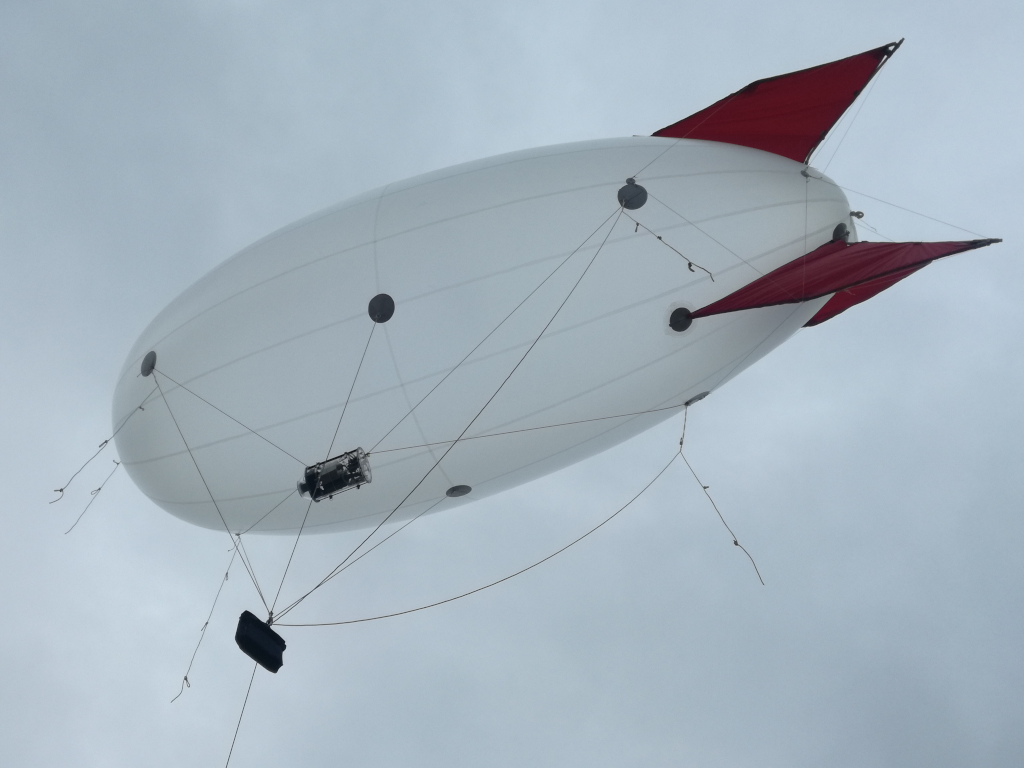
\includegraphics[width=0.8\colwidth]{img/balloon.png}
          \caption{The photo showing Backscatter Cloud Probe (BCPD) attached to a tethered balloon, deployed on October 1st, 2019 near Ny-\r{A}lesund, Svalbard.}
          \label{fig:01}
        \end{figure}

        The operation began at 18:00 UTC on October 1st, 2019, and lasted roughly two hours. The Back-scatter Cloud Probe (BCPD) measured a number of thermodynamic and microphysical properties of the advecting clouds at around 900 m above ground, with slightly varying altitude due to wind. The vertical trajectory of the instrument (and of the tethered balloon) can be seen in \Cref{fig:02} (black line).
      \end{block}

    \end{column}
    \separatorcolumn

    % Column 2
    \begin{column}{\colwidth}

      \begin{block}{Measurements}

        \begin{figure}
          \centering
          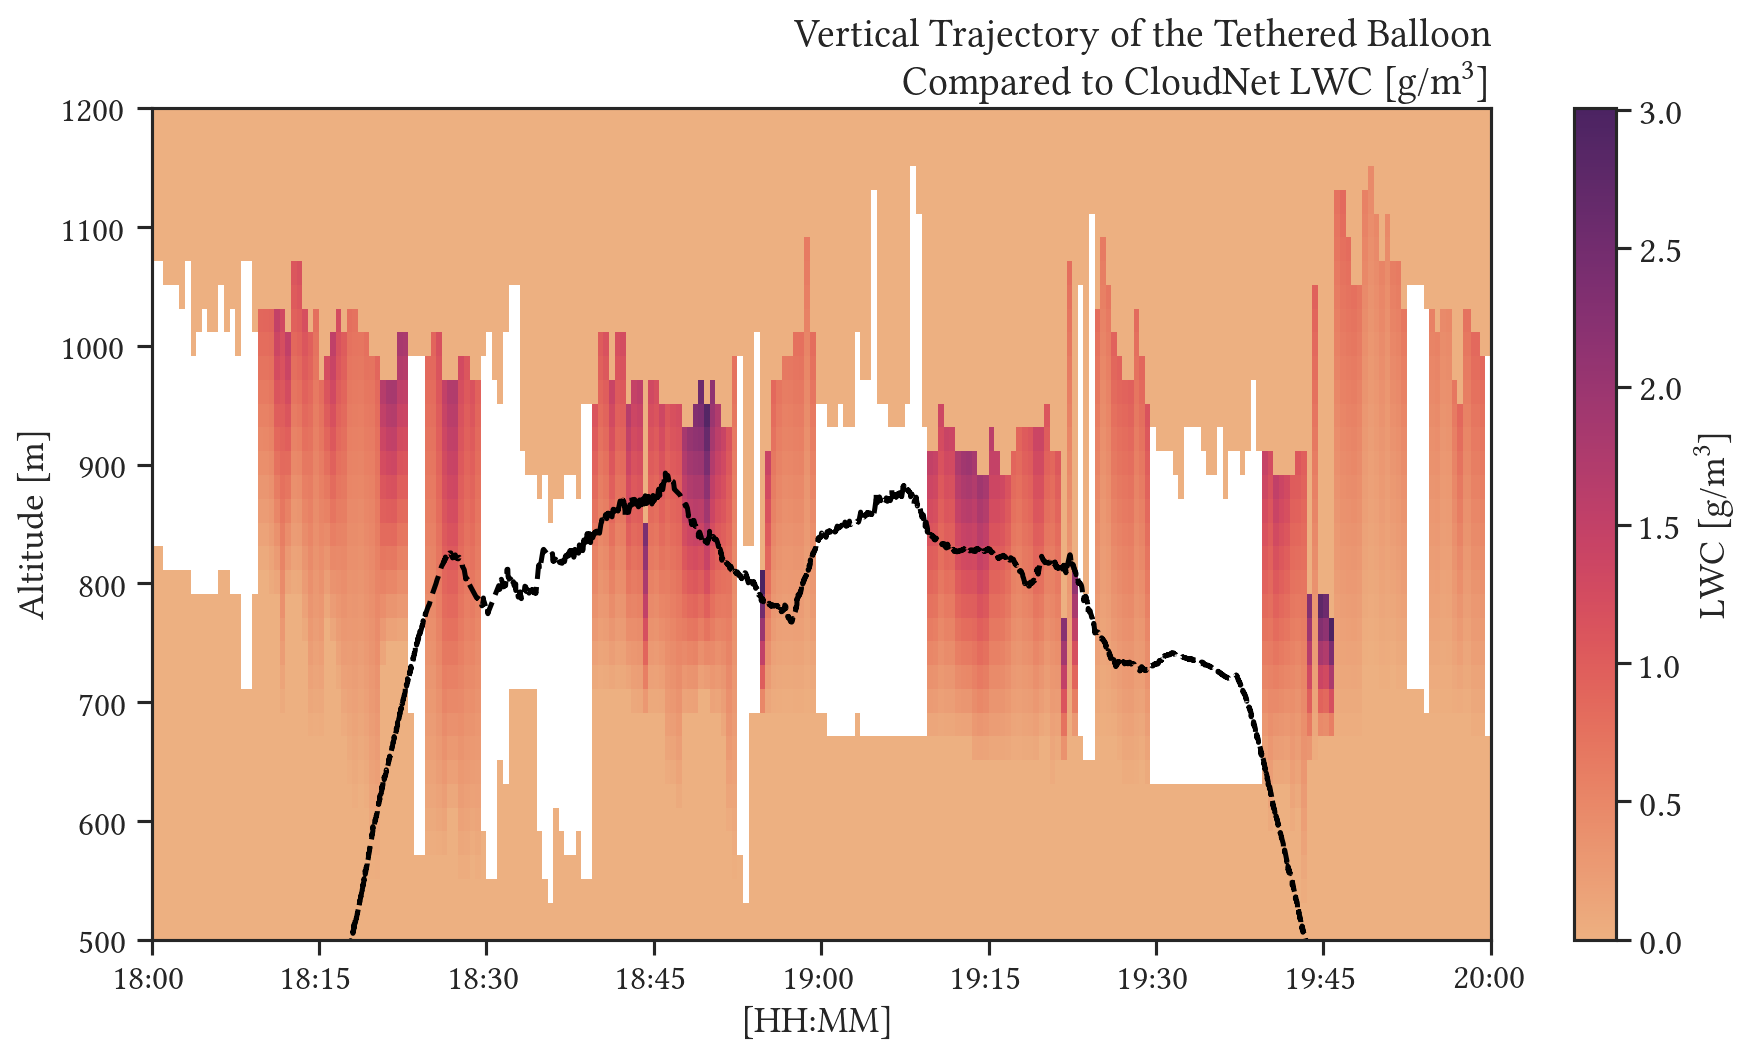
\includegraphics[width=0.95\colwidth]{img/ts_alt.png}
          \caption{The trajectory of the tethered balloon, compared to the liquid water content (LWC) in [g/m$^3$], reported by Cloudnet \cite{illingworth2007cloudnet}. The altitude recorded by the instrument on the tethered balloon is shown in black dashed line. The LWC values from the ground-based observation are displayed on a coloured map, with white regions indicating missing data.}
          \label{fig:02}
        \end{figure}

      \end{block}

      \begin{exampleblock}{Data Retrieval}

        We retrieved the liquid-water content (LWC) from ground-based remote sensing sites (Cloudnet) \cite{illingworth2007cloudnet}. The Cloudnet project provides vertical profiles of a number of cloud properties, including LWC. The vertical profile of LWC is mapped in \Cref{fig:02}. By tracking the varying altitude of the tethered balloon and mapping the corresponding LWC values, we could compare the liquid-water content measured by BCPD against the  ground-based observation (\Cref{fig:03}). Although the cloudiness of the surrounding air remained fairly consistent, the time-series of LWC reported by Cloudnet contains missing data, which is likely because clouds were not detected by the cloud radar at Ny-\r{A}lesund station \cite{illingworth2007cloudnet}. It is also possible that the presence of ice increased the uncertainty in the attenuation of ice reflectivity, but more work will be needed to estimate the properties of ice particles in the observed cloud.

        Since the BCPD was originally developed to be mounted on instrumented aircrafts, the assumptions made in processing the back-scattered signals into cloud properties (mainly LWC in this study) do not hold well with the measurements taken with the tethered balloon, mainly because the speed of the air passing through the sensor tends to be much slower on a tethered balloon. For this reason, LWC values were re-calculated by explicitly diagnosing the effect speed of the passing air. The 10-second measurements of LWC from BCPD (blue dots in \Cref{fig:03}) were further examined using Gaussian Process (GP) regression \cite{Rasmussen:2006vz}, which is a robust machine learning method that can estimate the underlying behaviour in the presence of uncertainties. It can also be used to estimate the confidence bound of the posterior distribution given noisy data, as shown in \Cref{fig:03}.

      \end{exampleblock}

    \end{column}
    \separatorcolumn

    % Column 3
    \begin{column}{\colwidth}

      \begin{alertblock}{Results}

        \begin{figure}
          \centering
          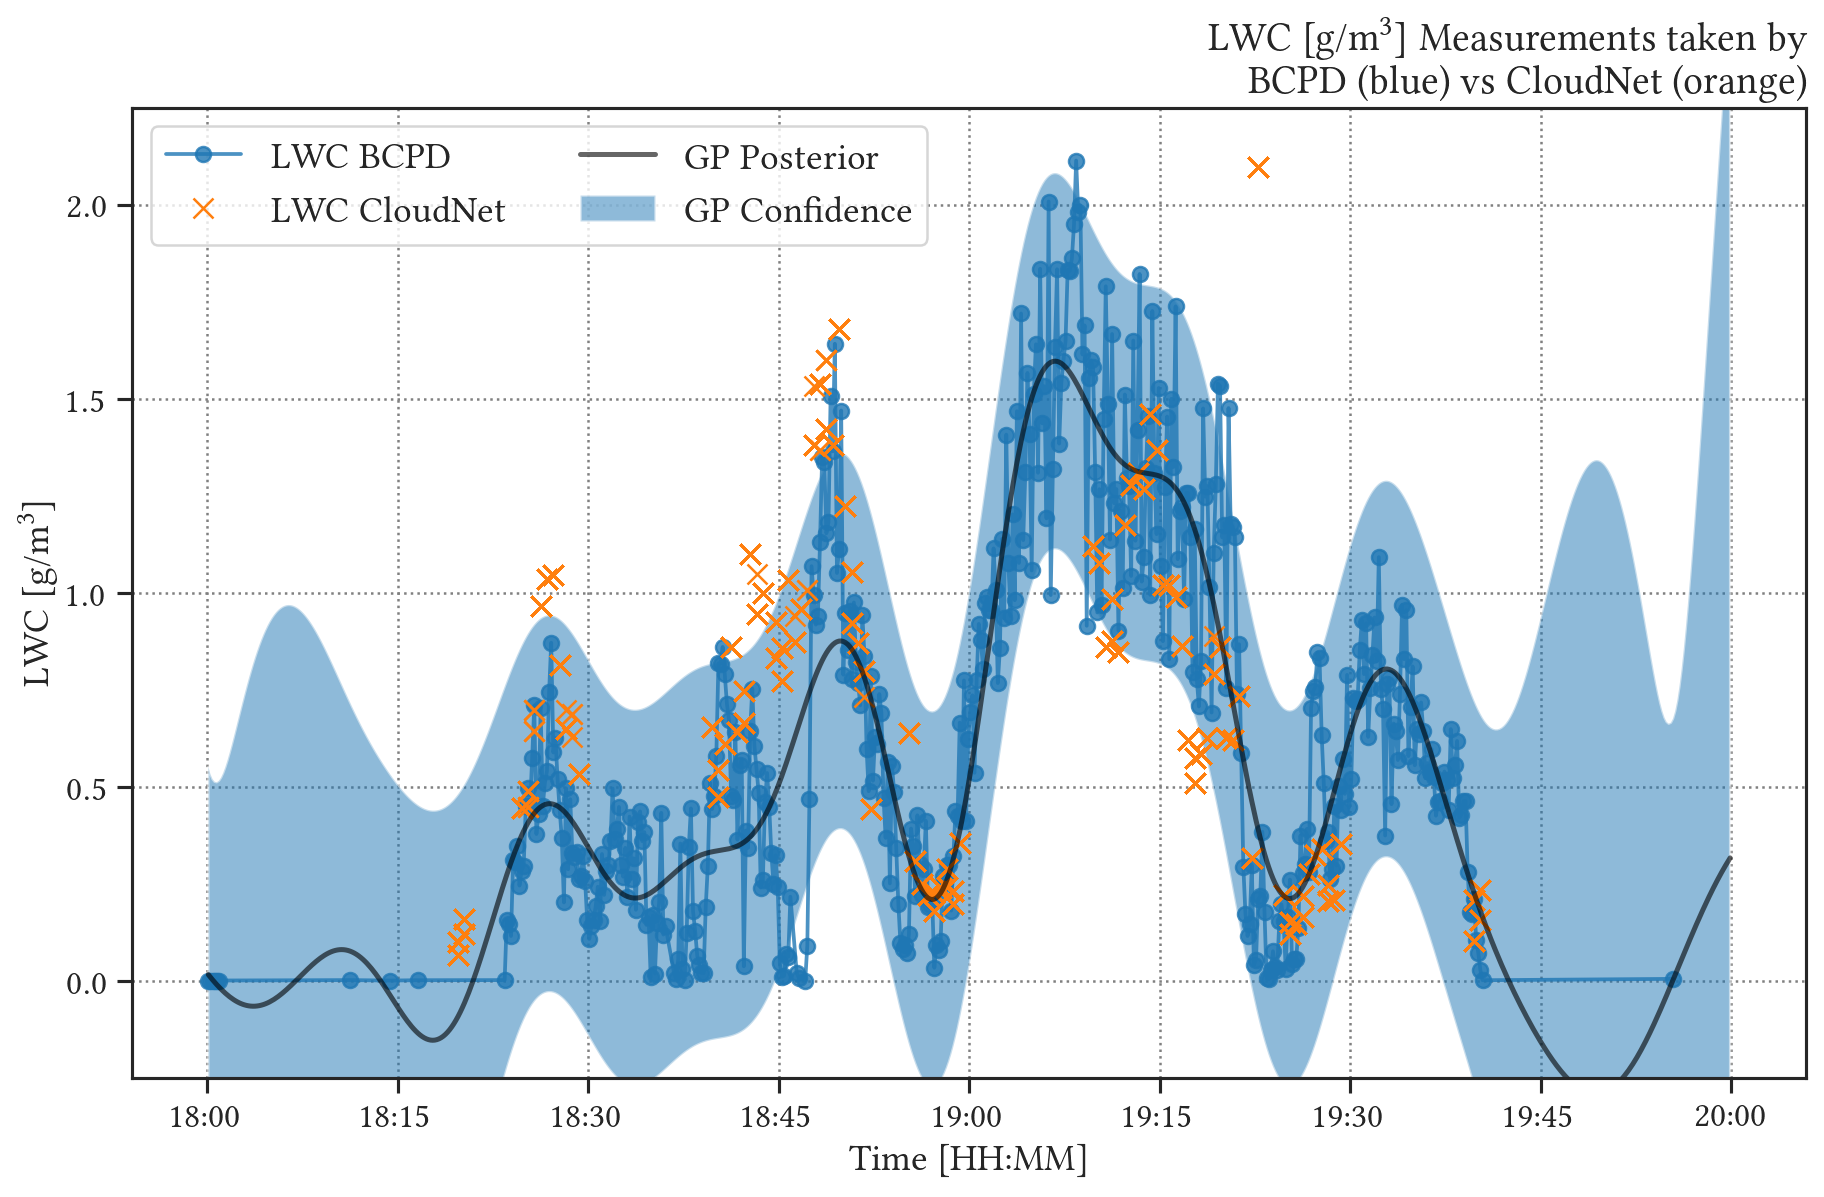
\includegraphics[width=0.95\colwidth]{img/ts_gp.png}
          \caption{ The time-series of liquid water content (LWC) [g/m$^3$] measured by BCPD on the tethered balloon (blue), and reported by Cloudnet \cite{illingworth2007cloudnet} (orange), as well as the mean posterior distribution from the Gaussian Process regression (black). The shaded region represents the 95\% confidence bounds based on the posterior distribution. }
          \label{fig:03}
        \end{figure}

      \end{alertblock}

      \begin{block}{Remarks}
        The liquid water content (LWC) of low-altitude arctic clouds were measured by Back-scatter Cloud Probe (BCPD) \cite{baumgardner2014ice, thomson2014compact} attached to a tethered balloon near Ny-\r{A}lesund, Svalbard. We compare these measurements to corresponding ground-based observations from Cloudnet \cite{illingworth2007cloudnet}, and confirm that the re-calibrated time-series data from BCPD are in good agreement with those from Cloudnet.

        A number of other cloud properties have also been measured during the tethered balloon experiment, such as cloud number concentration (NC), particle size distribution and polarization ratio. These observations will be used to further examine the properties of low-altitude arctic clouds, which will help improve our understanding of microphysical properties of arctic clouds. Having high-resolution measurements of cloud properties, especially the particle size distribution, will also be useful in examining the accuracy of current remote sensing operations.
      \end{block}

      \begin{block}{References}

        \nocite{*}
        \footnotesize{\bibliographystyle{plain}\bibliography{poster}}

      \end{block}

    \end{column}

    \separatorcolumn
  \end{columns}
\end{frame}

\end{document}
